\section{Possibility and necessity}

\begin{definition}[\textit{Possibility}]
    Possibility is another fuzzy measure that operates on sets. 
\end{definition}
A possibility measure is represented by the function $\Pi : \mathcal{P}(X) \rightarrow [0,1]$, and it adheres to the following properties:
\begin{enumerate}
    \item $\Pi(\varnothing)=0$ and $\Pi(X)=1$.
    \item $A \subseteq B \implies \Pi(A) \leq \Pi(B)$. 
    \item $\Pi(A)=\sup_{x \in A} f(x)$ where $A \subset X$. 
\end{enumerate}

A possibility measure can be uniquely defined by a possibility relationship $f:\textnormal{X} \rightarrow [0,1]$ such that:
\[\Pi\left(\bigcup_{i \in I}A_i\right)=\sup_{i \in I}\Pi\left(A_i\right)\]
This makes it possible to define $f$ as $\Pi\left(\{X\}\right)$ for all $x \in X$.
\begin{example}
    Consider the set $x=\{0,1,2,3,4,5,6,7,8,9,10\}$ and $\Pi({x})$, representing the possibility that $x$ is close to the value $8$:
    \begin{center}
        \begin{tabular}{|c|c|c|c|c|c|c|c|c|c|c|c|} 
            \hline
            $x$                         & 0 & 1 & 2 & 3 & 4 & 5     & 6     & 7     & 8 & 9     & 10    \\ \hline
            $\Pi\left(\{X\}\right) $    & 0 & 0 & 0 & 0 & 0 & 0.1   & 0.5   & 0.8   & 1 & 0.8   & 0.5   \\ \hline
        \end{tabular}
    \end{center}
    Now, let's compute $\Pi(A)$, which represents the possibility that $A$ includes an integer close to $8$. 
    For a given set $A=\{2,5,9\}$, we can calculate its possibility as follows: 
    \[\Pi(A)=\sup \left[\Pi\left(\{2\}\right), \Pi\left(\{5\}\right), \Pi\left(\{9\}\right)\right]=\sup\left[0,0.1,0.8\right]=0.8\]
\end{example}
\begin{definition}[\textit{Necessity}]
    Necessity is the dual concept to possibility and is defined as follows:
    \[\Pi(A)=\-N(\lnot A)\]
    It also satisfies the condition:
    \[\min\left[N(A),N(\lnot A)\right]=0\]
\end{definition}
These two measures, possibility and necessity, are connected by the following relations:
\begin{itemize}
    \item $\Pi(A) \geq N(A)$.
    \item $N(A) > 0 \implies \Pi(A)=1$.
    \item $\Pi(A) < 1 \implies N(A)=0$.
\end{itemize}
\begin{definition}[\textit{Confirmation degree}]
    The confirmation degree is a value that combines both possibility and necessity:
    \[C(A)=N(A)+\Pi(A)-1\]
    Negative values of $C(A)$ correspond to a disconfirmation degree.
\end{definition}

\subsection{Summary}
It is possible to demonstrate that if the focal set of elements for possibility (those with values of $m$ different from $0$) is composed of sets with a single element, then Bel and Pl have the same value. 
This value is equal to the sum of the probabilities of the elements of the set A to which they are applied, as given by $m$.

In the probabilistic model, evidence pertains to single elements, while in the possibility model, it can also be associated with sets. 
Both models have distribution functions, although they are normalized differently: in probabilities, they add up to one, while in possibilities, the maximum value is one.

In possibility theory, ignorance is expressed by assigning all the evidence to the universal set (i.e., anything is possible). 
In probability theory, on the other hand, it is expressed by distributing a uniform fraction of the evidence to each element (making each element equiprobable).
\begin{figure}[H]
    \centering
    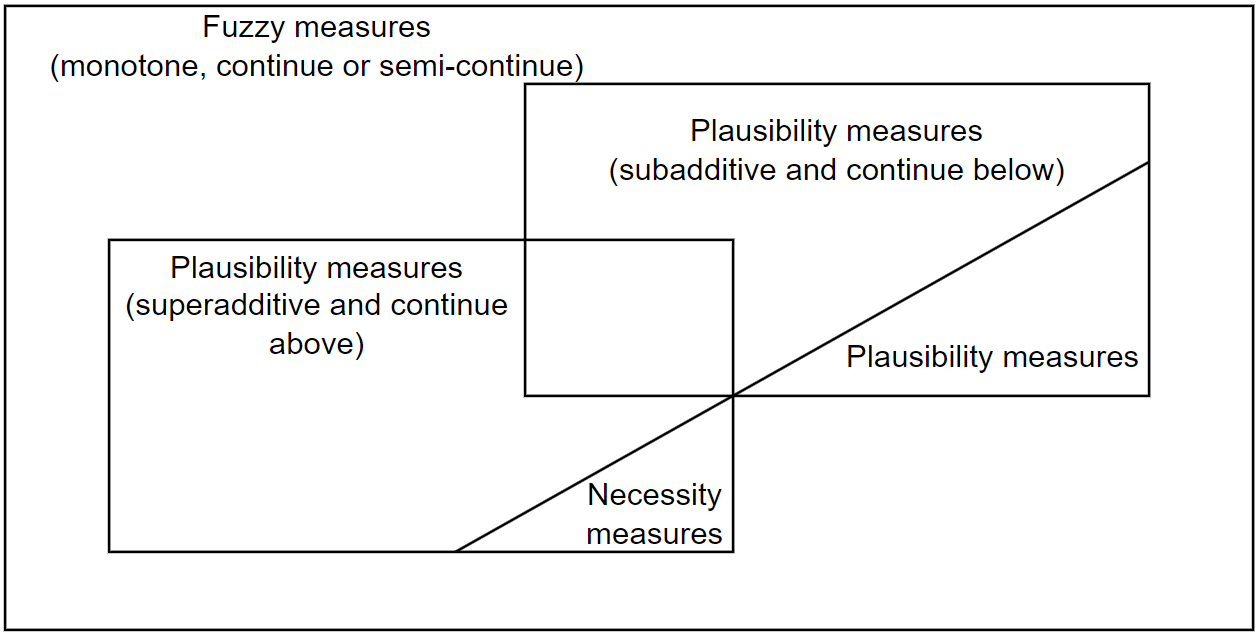
\includegraphics[width=0.75\linewidth]{images/measures.png}
    \caption{Inclusion relationships among fuzzy}
\end{figure}